\documentclass[conference]{IEEEtran}
\usepackage{graphicx}
\usepackage{amsfonts}
\usepackage{amssymb}
%\usepackage[spanish]{babel}
\usepackage{verbatim}
\usepackage{amsbsy}
\usepackage{amsthm}
\usepackage{amsmath}
\usepackage{siunitx}

\usepackage{algorithm}
\usepackage{algorithmic}
\usepackage[T1]{fontenc}		
\usepackage[utf8]{inputenc}
\usepackage{hyperref} 
\usepackage[super]{nth}
% correct bad hyphenation here
\usepackage{placeins} %para el FloatBarrier
\hyphenation{optical networks semiconductor IEEEtran}
%decimalpoint %decimales
%newtheorem{definition}{Definicion}[section]
%newtheorem{theorem}{Teorema}[section]
%newtheorem{lemma}{Lema}[section]

\theoremstyle{definition}
\newtheorem{definition}{Definition}[section]
\newcommand{\ts}{\textsuperscript}
% \newcommand{\bol}{\boldsymbol}

\renewcommand{\abstractname}{\center\large Abstract\\}
\let\oldabstract\abstract
\renewcommand\abstract{%
  \begingroup
  \let\textit\relax
  \oldabstract
  \endgroup
  \bfseries
}

\usepackage{lipsum}


\begin{document}

% paper title
\title{Automatic tuning of adaptive PID controllers using an artificial neural network}


% author names and affiliations
% use a multiple column layout for up to three different
% affiliations
\author{\IEEEauthorblockN{Soleiman N. Anwary, Charles Rigby}
\IEEEauthorblockA{Department of Process Systems Engineering, Imperial College London\\
\{sna314, cwr17\}@imperial.ac.uk}
}



% make the title area
\maketitle

\begin{abstract}
Although the analysis of data is a task that has gained the interest of the statistical community in recent years and whose familiarity with the statistical computing environment, they encourage the current statistical community (to students and teachers of the area) to complete statistical analysis reproducible by means of the tool R.
However for years there has been a gap between the calculation of matrices on a large scale and the term "big data", in this work the Normalized Cut algorithm for images is applied. Despite the expected, the R environment to do image analysis is poorly, in comparison with other computing platforms such as the Python language or with specialized software such as OpenCV \cite {OpenCV}. \\
Being well known the absence of such function, in this work we share an implementation of the Normalized Cut algorithm in the R environment with extensions to programs and processes performed in C ++, to provide the user with a friendly interface in R to segment images. The article concludes by evaluating the current implementation and looking for ways to generalize the implementation for a large scale context and reuse the developed code.

\textit{Key words: Normaliced Cut, image segmentation, Lanczos algorithm, eigenvalues and eigenvectors, graphs, similarity matrix, R (the statistical computing environment), open source, large scale and big data.}\end{abstract}

\IEEEpeerreviewmaketitle


\section{Introduction and motivation}



The statistical recognition of patterns, and in particular the analysis of images, is a stimulating field of study where statistics and computer science coexist. In recent years the environment of statistical computing and programming language R \cite{R} has increased its presence in statistical analysis and is even used in big data contexts, on the other hand, image analysis is an area that continues to motivate investigation.\\
As a counterpoint to what is expected, since image analysis uses different statistical learning techniques (both supervised and non-supervised), the R environment has few tools for image analysis, as can be seen when reviewing the entry of 'MedicalImaging' in its Task View, in front of other specialized tools such as OpenCV \cite{OpenCV}. On the other hand, there are scientific computing environments that integrate some tools to analyze images, but their capacities are reflected in their commercial price, for example MatLab \cite{MatLab}. \\
%%%%%
The above, together with the fact that image segmentation is a final objective and sometimes only an intermediate step in other investigations, in this work an image segmentation application is developed using the Normalized Cut algorithm, which we will refer to in the following as \textit{Ncut}. In order to provide users and developers of the R language with an implementation of the \textit{Ncut} algorithm (which does not exist in OpenCV and other scientific computing environments), two programs were coded; each contains a file with extension .R that determines it as an R language code as well as a file with extension .cpp that is a C ++ language code that uses stable C ++ language libraries to perform calculations and optimal storage of matrices;
one for grayscale images and one for RGB images available in the github author's personal \cite{github}  \url{https://github.com/fou-foo/MCE/tree/master/Second/AnalisisNumericoYOptimizacion/Miniproyecto} respectively the files are ''W\_float.cpp'' and ''mini\_cut\_float.R'' for grayscale images and ''W\_RGB\_float.cpp'' and ''mini\_Ncut\_RGB\_float.R'' for images on RGB channels (which is easily adaptable to images with more channels). Details on implementation are discussed in the last subsection of section ''II. Workflow ''of this report. \\
With the above, an easy-to-use open-source tool is provided, particularly in the R environment, although the .cpp code can be exported to other computing environments, for the Ncut algorithm, which provides the basis for future statistical computing developments. The product developed allowed to segment a set of images from the personal profile of the author of the Facebook \cite{Facebook} platform, whose results are reported in this work. \\
The organization of the present work is as follows: in the section 'II. Workflow" is explained in a general way in which the Ncut algorithm that was used in this work consists, as well as its relation with the Lanczos algorithm, later the implementation of the algorithm is detailed so that it is easy to use in the R environment.In the section ''III. RELATED WORKS'' we report the research carried out on the lack of implementations of both the Ncut algorithm and the Lanczos algorithm in different architectures (which makes the need for an own implmentation tangible) such as tools dedicated to the big data context (such as Apache Hadoop \cite{Hadoop} and Apache Spark \cite{Spark}) where the author sees an area of opportunity for massive image analysis, on the other hand, in large-scale matrices there are implementations in MPI such as ScaLAPACK \cite{ScaLAPACK} of the Lanczos algorithm, however, they do not implement higher-level routines such as Ncut. We conclude this section by commenting on tools that we consider medium-term to be useful for large-scale scientific computing such as the programming language Elixir \cite{Elixir}. \\
Then in the section "IV. Experiments and Results" are shown (and in some images are detailed) the results of the image segmentation realized with the own implementation. The section concludes with the benefits and limitations of the implementation to obtain a "good" image segmentation. Later in the section "V. Conclusions" we summarize the discoveries learned and evaluate the methodology used. Finally, the "Appendix" section proposes future works of improvement of the implementation, within the open-source context, to segment images of greater resolution and size to those addressed in this work, as well as the possible extension to other statistical learning techniques with the purpose of reusing the code already developed and future. \\



\section{Methods}

\section{Mathematical and Computational Aspects}
We are addressing the problem of tuning parameter optimisation using a surrogate machine learning model. We are using a quadratic approximation to the actual dynamics of the system. For this problem to be soluble the surrogate model has to be convex and all the constraints must also be convex such that the problem overall is convex. \\
\theoremstyle{definition}
\begin{definition}
\textit{A function f}: $\mathbb{R}^n \rightarrow \mathbb{R}$ \textit{is convex if and only if its domain is a convex set $\forall$ $x, y$ and all $\lambda \in [0,1]$. } 
\end{definition}

A multivariate quadratic function such as the surrogate model
\begin{equation}
    f(x) = x^TQx + c^Tx,
\end{equation}
is convex if and only if $Q \succcurlyeq 0$. This is important because it means that the quadratic coefficients of the surrogate model have to be constrained to non-negative values. So by defining Q to be a symmetric matrix and the constraining the quadratic term coefficients to be non-negative we ensure all eigenvalues of the matrix are positive and as such the matrix $Q$ is positive semi-definite which keeps the optimisation problem convex. Most importantly, a convex system means any local minimum found is also a global minimum. 


%--------------------------RESULTS AND DISCUSSION------------------------------------
\section{Results \& Discussion}
\subsection{Optimisation of a 2D Control System}

When optimising a control system we first had to segment the problem. The majority of dynamic systems are controllable using a P and I control system [Reference]. With this in mind, we pose the hypothesis: the algorithm should come to the conclusion that the majority of systems tested are PI-controllable. Indeed what we observed was that both linear and non-linear system dynamics were controllable and converged onto a set point; a number of set points were used to test model robustness and in each case the model presented a converging system response. We can see Figure X shows system responses for the optimal set of tuning parameters, $k_p$ and $k_i$  as determined by the surrogate model optimisation. Several iterations of the model were plotted on the same axis to show how the algorithm parses through the mesh of tuning parameters generated. The darker lines represent later iterations and the latest updates to the optimal response. The following were used as benchmark dynamic systems to test the model performance:
\begin{equation}
\frac{dx}{dt} = 2x +u \quad \textrm{and} \quad \frac{dx}{dt} = x^2 + u
\end{equation}
It is important to note the algorithm is designed to work on unknown system dynamics; the outputs of the system would be gathered and fed into the algorithm as an input. This would be used by the model to fit an approximate surrogate function and find the optimal tuning parameters.\\
The cost function $\phi$ is evaluated at each iteration and plotted over the parameter vector space to visualise the surface. We do this in a 3-dimensional plot of $k_p$ against $k_i$ and $\phi$. The value of $\phi$ is broken into percentiles and categorised in the plot using a continuous colour scale. It can be seen the cost function $\phi$ predicts the optimal value of $\boldsymbol \pi$ to be in the region with low $k_i$ and high $k_p$ values. The sample space in the parameter mesh is cubic and this is seen in the plot. The surrogate function $\phi_{approx}$ predicts the optimal $\boldsymbol \pi$ to be at $(5,5)$. This is not completely consistent with what the cost function predicts. This may be because the surrogate model is sampled far more around that point and as such a greater weight is given for that set of values as the optimum $\boldsymbol \pi$ [CLARIFY THIS WITH ANTONIO]. A higher density plot of phi was generated to test this and indeed the optimum predicted by the surrogate function moved closer to the darker red region where $\phi$ is minimised [figure reference].
Furthermore, while low values of the integral term are preferred - which controls how smooth the system response is - a zero value for $k_i$ is not. Without any integral action the system response starts oscillating and often results in a steady state error. We therefore suggest that a PI-control system is sufficient for most linear and non-linear systems with first order dynamics. 

\subsection{$\phi_{approx}$ vs. $\phi$ Fit }
We investigated the agreement between the surrogate function $\phi_{approx}$ and the cost function $\phi$ in Figure X. Comparing the contours to the 3-dimensional scatter plot for $\phi$ in Figure X shows us that there is a large flat region before the surface shows curvature. This is seen in the contour plots. More specifically, there are three cases which were isolated for analysis: a) system convergence, b) divergence and c) fast oscillatory system response. In case a) we can see that the contour starts curving to a minimum which is in a region with a high $k_p$ and low (and non-zero) $k_i$ value. This is consistent with the predictions from the cost function alone. We can see the system reaches a steady state set point value preset at 15 for this experiment. Case b) presents a case where the contour is approaching a point which is in a region with low $k_p$ and high $k_i$. It is clear that when the proportional gain is not large enough the system is not only slow to respond (large rise time) it is also unable to reach a steady state value and therefore stability. The final case is the last iteration of the experiment and shows that a possible system response is one with both $k_p$ and $k_i$ at the boundary of the active constraints set; here we observe large initial overshoot and initial oscillations which are brought about by the larger integral term. 

\subsection{Optimisation of a 3D Control System}
We extended the PI-control parameter optimisation to the 3D case by also considering a derivative term, $k_d$. Figure X shows various system dynamics and how the model handled the optimisation to achieve a steady state system response for both linear and non-linear system dynamics. Once again we used several set point values to test the model and system response convergence. All tests showed the model successfully corrected for the step input error and brought the system back to the set point. There are several values of $\boldsymbol \pi$ which led to a sub-optimal response where the system slowly diverged from the set point. However, the last batch of iterations show that the most intensely coloured blue lines belong to the group of $\boldsymbol \pi$ solutions which yield a steady state system response. It was also important to understand how the cost function behaved across the parameter space. Figure X shows a 4-dimensional plot of the parameters $k_p, k_i, k_d$ and the value of $\phi$ normalised as a percentile as the 4\ts{th} dimension which is shown as colour in this instance. We can see that once again a high value of $k_p$ and low but non-zero values of $k_i$ are preferred by the model for linear and simple non-linear dynamics. The parameter $k_d$ is often very close to or in fact \textit{zero}. This reinforces the model's PI-control preference; it suggests that a proportional gain and a small integral error correction mode are sufficient to control most systems effectively. Furthermore, the surrogate approximate function $\phi_{approx}$ attempts to find optimal values for $\boldsymbol \pi$ in the region where the derivative term is zero, and the proportional and integral terms are equal because the model samples heavily in that region. This suggests that there is a compromise that has to be achieved for the surrogate model. It can either try to approximate the system dynamics in small local spaces which would improve the fit between $\phi$ and $\phi_{approx}$ or it can approximate the dynamics globally which means that $\phi_{approx}$ cannot be accurate across the whole domain. The model is designed to be memoryless - upon each iteration the model does not retain any state space variables describing the system or the tuning parameters which were used in the previous iteration prior to bound reduction. As a result, the approximate surrogate function inherently will not be able to approximate the system dynamics equally well over the entire space. 

\subsection{Multiple Input Multiple Output Control System (MIMO)}

When designing the control algorithm it was important to consider use-case scenarios for its application. One such use-case is in biochemical processes. Biochemical processes utilise biological microorganisms to produce chemical derivatives and high-value products otherwise too complicated to obtain through physical chemical modes. However, the complex interactions between the substrates in metabolic pathways and the culture fluid dynamics makes bioprocess control particularly challenging to control [Reference Rio del Chanona, Reinforcement learning for batch bioprocess optimization]. System-wide or plant model dynamics cannot meaningfully be obtained for such processes and as such they must be treated as black-box models. Often there are multiple controlled variables such as pH, feed stock concentration, product concentration, temperature, pressure and flow rate; many of these parameters are dependant on each other and as such a control system which can allow communication between multiple controllers which correct related system states is important. \\
As such we have developed an artificial neural network (ANN) for multiple controllers which are linked to each other by a surrogate model function - in this case $\phi_{approx}$. This surrogate model will allow the controllers to communicate and compromise on the optimisation of the tuning parameters to reach system stability. The tuning parameters make up the weights of each distinct error term in the input layer, allowing the controllers to generate control functions as the output. With that in mind we tested the extended model on two controllers and applied it to both linear and non-linear systems,
\begin{align}
    \dot{x_1} &= 2x_1 + x_2 +2u_1 - u_2 \\
    \dot{x_2} &= x_1 + 2x_2 - 2u_1 + 2u_2.
\end{align}

Figure X shows both system dynamics were brought to stability using the optimised tuning parameters. The history of how the model reached the optimal system response is shown. Upon addition of disturbance to the environment and noise to the controllers we optimised the tuning parameters and achieved stability for both the linear and non-linear system as is shown in part b) of Figure X. This model can be tested for $n$ number of controllers and the optimisation algorithm will coordinate the controllers since the optimiser adjusts the weights of the proportional, integral and derivative term for all controllers simultaneously. This makes the surrogate function a communication pathway to reach a globally optimal solution while exerting control on all system variables.

\subsection{Limitations \& Complexities}
\subsubsection{Stochasticity}
When developing this blackbox optimisation model we added disturbance and noise to the system environment and control system itself, respectively. This was done to test the robustness of the algorithm to sudden and small changes and simulate a stochastic version of the model. A non-robust controller would explode the derivative term in response to the uneven characteristics of the system response if the tuning parameters are not optimised correctly. Interestingly, we saw that the model was able to bring linear and non-linear systems to stability but at the costs of removing the derivative term entirely. This may be because the derivative term, while reducing the initial overshoot of the system, would become too sensitive to disturbance and noise from the environment and controller, respectively. We used a frozen Gaussian probability density function (one where the mean and standard deviation is fixed for each random variable generated) to add the complexity of disturbance and noise as given by,
\begin{equation}
    p(x) = \frac{1}{\sqrt{2\pi \sigma^2}} \exp{-\frac{(x-\mu)^2}{2\sigma^2}}
\end{equation}

\noindent Where $\mu$ is the mean and $\sigma$ is the standard deviation. A mean of $\mu = 0$ and standard deviation of $\sigma = 0.2$ were used. 

\subsubsection{Hyperparameter Optimisation}
There were several hyperparameters which we did not yet optimise for in this model. These include the number of iterations the neural network needs to run to each an optimum value, the size of the network itself, and the activation function for the optimisation. Blackbox optimisation problems rapidly become computationally expensive. This is apparent when looking at the architecture of the ANN for the MIMO system. Each controller commands a set of six coefficients and three tuning parameters in the surrogate function and with a sample space as small as two samples per tuning parameter the space grows exponentially by $(2n)^i$ where $n$ is the number of nodes and $i$ represents the dimensionality of the vector space, 3, in this case. As such we only tested the MIMO system using two controllers as we were running all simulations on a 2014 \SI{2.2}{GHz} Quad-Core i7 processor chip. \\
Currently, we are using a linear activation function in the PID controller i.e. the $u$ function. This means that the current neural network cannot stack several layers because irrespective of the number of layers in the neural network the activation of the output layer is simply going to be a linear combination of the input of the first layer. This can be overcome by replacing the linear activation function with a non-linear function such as a Sigmoid function or a hyperbolic tangent function like below, 
\begin{align}
    s(x) &= \frac{1}{1 + e^{-x}} \\
    f(x) &= \tanh(x) = \frac{1}{1+e^{-2x}}.
    \end{align}
\vspace{3mm}

\section{Outlook \& Further Work}
\subsubsection{Non-linear Activation Function}
As previously alluded to, it would be important to ascertain the model's behaviour with a non-linear activation function; this would be in pursuit of creating a better fit between the system dynamics and the approximate surrogate function globally across the entire sample domain.
\vspace{2mm}
\subsubsection{Step Change Input}
It would be most curious to train the neural net on a set of different disturbances and step input changes so that the model is able to handle large changes in the environment more effectively. This would involve prediction of optimal tuning parameters for specific step changes. 
\vspace{2mm}
\subsubsection{Gaussian Processes}
In this paper we have explored the use of a convex quadratic function to approximate the system dynamics. However, studies have shown that using Gaussian processes in place of a quadratic function can yield better results for global optimisation problems [Osborne, M. A., Garnett, R., \& Roberts, S. J. (2009). Gaussian processes for global optimisation]. Gaussien Processes are a generalisation of the Gaussian probability distribution. While probability distributions can describe random variables, Gaussian processes (which are stochastic bu definition) describe properties of functions over a finite space [Rasmussen Book]. One of the reasons why Gaussian processes may be a better fit for this than a quadratic function might be because the presence of significant stochastic uncertainties in a system environment can lead to closed-loop performance and uncontrollability issues. GPs can be used to formulate nonlinear constraints for non-linear systems and thus improve control performance [Bradford, 2018  Stochastic Nonlinear Model Predictive Control Using Gaussian Processes]
\vspace{2mm}
\subsubsection{Reinforcement Learning - Q-learning}
    
































\subsection{Details of the implementation (in particular in the R language)}
The R programming language in particular has challenges in the application of the \textit{Ncut} algorithm due to the following reasons:
\begin{enumerate}
\item The representation of the images and in general of the floating point numbers correspond to the standard of \textit {double} of the C ++ language
\item R loads all the objects with which you work in RAM.
\end{enumerate}
However the sparse matrices are easy to handle in the R. environment.\\
Following the diagram in figure 1, the disk reading was did with the package \textit{imager} \cite{imager} which represents the images as a 4-dimensional array where the first two dimensions correspond to the height and width of the image, and the fourth dimension corresponds to the channels available to the image. This 4-dimensional representation uses the type \textit{numeric} of R that corresponds to 64-bit C ++ data type \textit{double}. In cases where it is required to resize the image, it was done with the same package of R. \\
To counteract point (1) above, the calculation of the $ W $ matrix is done in C ++ by restricting the type of data between operations to the type \textit{float}, for which the Rcpp \cite{Rcpp} package is used and to store the matrices in a sparse matrix format, the RcppEigen \cite{RcppEigen} package is used, which allows to interact with the Eigen library of the C ++ language, so that the output of the C ++ code is an array $ W ^ * $ symmetric, positive semi-definite and of the sparse type that incorporates the necessary information to solve the problem of the eigenvalues of equation (3).
In particular, the program that segments images with more than one channel uses the RcppArmadillo \cite{RcppArmadillo} package, which has an interface to use the C ++ Armadillo linear algebra library, to use 3-dimensional arrays (in this point is important to mention that the real implementation requires changes to the header of the file \textit{RcppArmadillo.h}, increase the line ''\#include <RcppEigen.h>'' as the default installation and the process of \textit {attach} (innate of the R language) conflicts the headers \textit {RcppEigen.h} and \textit {RcppArmadillo.h} as both refer to the \textit {Rcpp.h} header, however when add the mentioned line a single header includes a others in a single invocation and \textit {attached file}). \\
Up to this point we used the C ++ language for the calculation of $ W $, notably improving the execution time compared to doing it in R, besides saving memory space of 50 \% when using only the data type \textit {float } instead of \textit {double} \\
To counteract point (2) of the previous list, objects that are no longer required are explicitly removed from the environment and we explicitly called the garbage collector. The package for the fourth step uses a function of the Rspectra \cite{RSpectra} package, which is an interface to the Spectra library developed in C ++ similar to the ARPACK library (developed in Fortran), which refers to a C ++ implementation of the Lanczos method implicitly restarted and to obtain the smallest eigenvalues in the place of the large ones, which use the method of change around the zero in place explicitly, the matrix $ W ^ * $. \\
The fifth step that consists in applying kmeans on the eigenvectors obtained previously, was done with the implementation of the base kernel of R with 50 iterations and fixing the seed in both cases to provide reproducibility to the experiment, finally the application of the segmentation corresponds to a convolution of matrices between the original image, after having been resized if necessary, and the arrangement of the segmented pixels. In the case of images with three channels, this convolution maps by channel to the original value of the pixel to zero, or multiplies it by 0.5 or leaves it intact depending on which segment it belongs to.
\section{Related jobs}
In the previous section we detailed an implementation to segment images using the \textit {Ncut} algorithm that depends strongly on the implementation of the RSpectra \cite {RSpectra} package of the implicitly restarted Lanczos method, which, as we mentioned earlier, invokes an implementation in C ++ of its analog in Fortran of the classic ARPACK \cite {Arpack} library to solve the problem of finding the eigenvectors associated with the smallest eigenvalues of a positive and scattered semidefinite symmetric matrix. However, the current implementation is limited in terms of the size of the $ W $ matrix, which is why we resort to resizing the images in sizes approximately greater than $ 138 \times 138$. \\
In a large-scale context the ScaLAPACK \cite {ScaLAPACK} library implemented a routine that solves the problem of values and eigenvectors for the symmetric case (such as the one we attacked), however in a big data context there are friendly implementations, even with a API to the Python language (see \url {https://spark.apache.org/docs/2.3.0/mllib-dimensionality-reduction.html}), of the SVD decomposition (considering only the largest singular values ) whose implementation is detailed in \cite {MatrixSpark}, with this work (and its current implementation of the QR decomposition) or with the implementation of the inverse of a matrix in the Spark environment proposed in \cite {Sparkbased} makes it plausible to scale the problem and the segmentation of images using the \ textit {Ncut} algorithm, however, this requires a new data and computing architecture. \\
On the other hand we hope that programming languages that are born as functional and concurrent as Elixir \cite{Elixir} will develop robust libraries for scientific computing in the medium term, since today the language has a linear algebra library, without However, it is still in a state of development \cite {ElixirLib}, as we can see by noting that its implementation of the inverse of an 'inv' matrix uses Gaussian elimination and brute force.
\section{Experiments and results}
The current implementation we shared of the algorithm \textit {Ncut}, was applied to a set of images from the author's Facebook profile. The experiments are reported in the following Table I, making reference to each image with a number and the average time of the execution in the image. The experiments were performed on an Asus GL553VD machine with 8 GB of RAM (but due to the configuration of the Windows 10 operating system) it is only possible to fully use 6 of these 8 GB, with an Intel Core i7-7700HQ processor (with 8 logical cores) at a speed of 2.5GZ. \\
During the execution times, and part of the development, we were able to estimate the amount of RAM a PC requires to execute the current implementation of \textit {Ncut}, which is approximately 4 times the space required to store the array $ W $ , this because at some point it is required to have in memory two matrices additional to the $ W $ matrix of the same dimensions and same characteristics, in addition to the memory that the Lanzos implementation uses to be made.
\begin{table}[h]
\begin{center}
\begin{tabular}{c|cccccc}
\hline  \begin{tabular}{@{}c@{}}Image's\\ number\\ and name \end{tabular}  &\begin{tabular}{@{}c@{}}Original\\size\end{tabular}& \begin{tabular}{@{}c@{}}Analyzed\\size\end{tabular} 
%(después de redimensionarla) 
& \begin{tabular}{@{}c@{}}Execution\\time\\ grayscale\\(mins)\end{tabular} & \begin{tabular}{@{}c@{}}Execution\\time\\ RGB\\(mins)\end{tabular} &  \begin{tabular}{@{}c@{}}Matrix\\size\\$W$\\(MB)\end{tabular}\\ \hline
1: Cell.jpg	     &100	$\times$ 69        & 100$\times$ 69 & 22.3 secs&	17.6 secs & 133.1\\
2: los\_amantes.jpg  &397 $\times$ 504     & 397$ \times$ 504   & 2.1 &2.4& 429.1\\
3: foo.jpg	&528 $\times$	528 &  132$\times$132	& 4.6&5.9 &855.2\\
4: guapa.jpg &970$\times$	720 & 100$\times$	180	&4.6& 4.9& 330.1\\
5: fer.jpg &533$\times$960 &100$\times$180 & 8.8 & 7.0 & 874\\
6: brindis.jpg	&1280$\times$960 & 160$\times$120 & 13.7 &7.1& 1000\\
7: foo\_clau.jpg &1280$\times$720&	104$\times$180 & 7.0& 8.1& 954.6\\
8: f002.jpg&960$\times$960&138 $\times$138& 16.9&8.9&1000\\
9: frascos.jpg&2048$\times$1152&180$\times$103&7.5&4.1&943.4\\
10: foo3.pjg&960$\times$960&138$\times$138&11.3&12.4&1000\\
%11: luis.jpg&2048$\times$1365&165$\times$110&3.8&10.2 &926.7\\
11: bicis.jpg&1280$\times$960& 160$\times$120&31.5&33.5&1000\\
%12: santa\_lucia.jpg&2048$\times$1152&182$\times$102&8.1&7.5&943.8\\
12: mariposa.jpg&2048$\times$1151&178$\times$100&5.9&3.3&863\\
13: filo\_liz.jpg&2048$\times$1152& 182$\times$102&7.9&7.0&943.8\\
14: marco.jpg&2048$\times$1365& 166$\times$110&5.4&4.7&933\\
\hline
\end{tabular}
\caption{Summary of the execution of the algorithm \textit {Ncut} in the set of sample images. Note that from image 2 all the images were resized.}
\label{tresultados}
\end{center}
\end{table}
\FloatBarrier
Figure 2 (from top to bottom) shows the results obtained when selecting images 1 to 5 using the two sets of channels (grayscale and RGB) after being resized to the sizes described in table I. It is interesting to note that the results are ideal for images 1 and 5, on the other hand, for images 3 and 4 they can be identified by themselves, however, in image 2 as it is a photograph of a pencil, the clamps that hold up are easily identified the sketch and it is not until the segmentation with two eigenvectors (right) that is identified as the whole sketch as a single differential set of the tweezers. \\
In figure 3 (from top to bottom) the results obtained by segmenting the images 6 to 10 using analogously notation to figure 2 are shown. It is interesting to note that the results are consistent when recognizing people from the background, for example figure 10 and 8 (where the person is detected even in the segmentation that uses only an own vector and achieving greater detail when using more components) however in image 6 the segmentation in RGB is only able to identify the clothes of the person in green . When viewing the image 9 we noticed that in particular the implementation is delicate recognizing glass objects however it distinguishes well other materials such as plastic. In particular of the results of Figure 6 and 7 we can see that the light conditions affect the performance of the implementation which suggests an improvement in the preprocessing for future work. \\
\begin{figure}[htbp]
\center{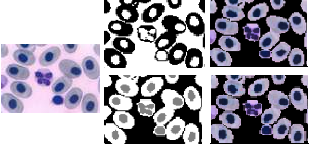
\includegraphics[width=5.0cm]{res_cel.png}}
\center{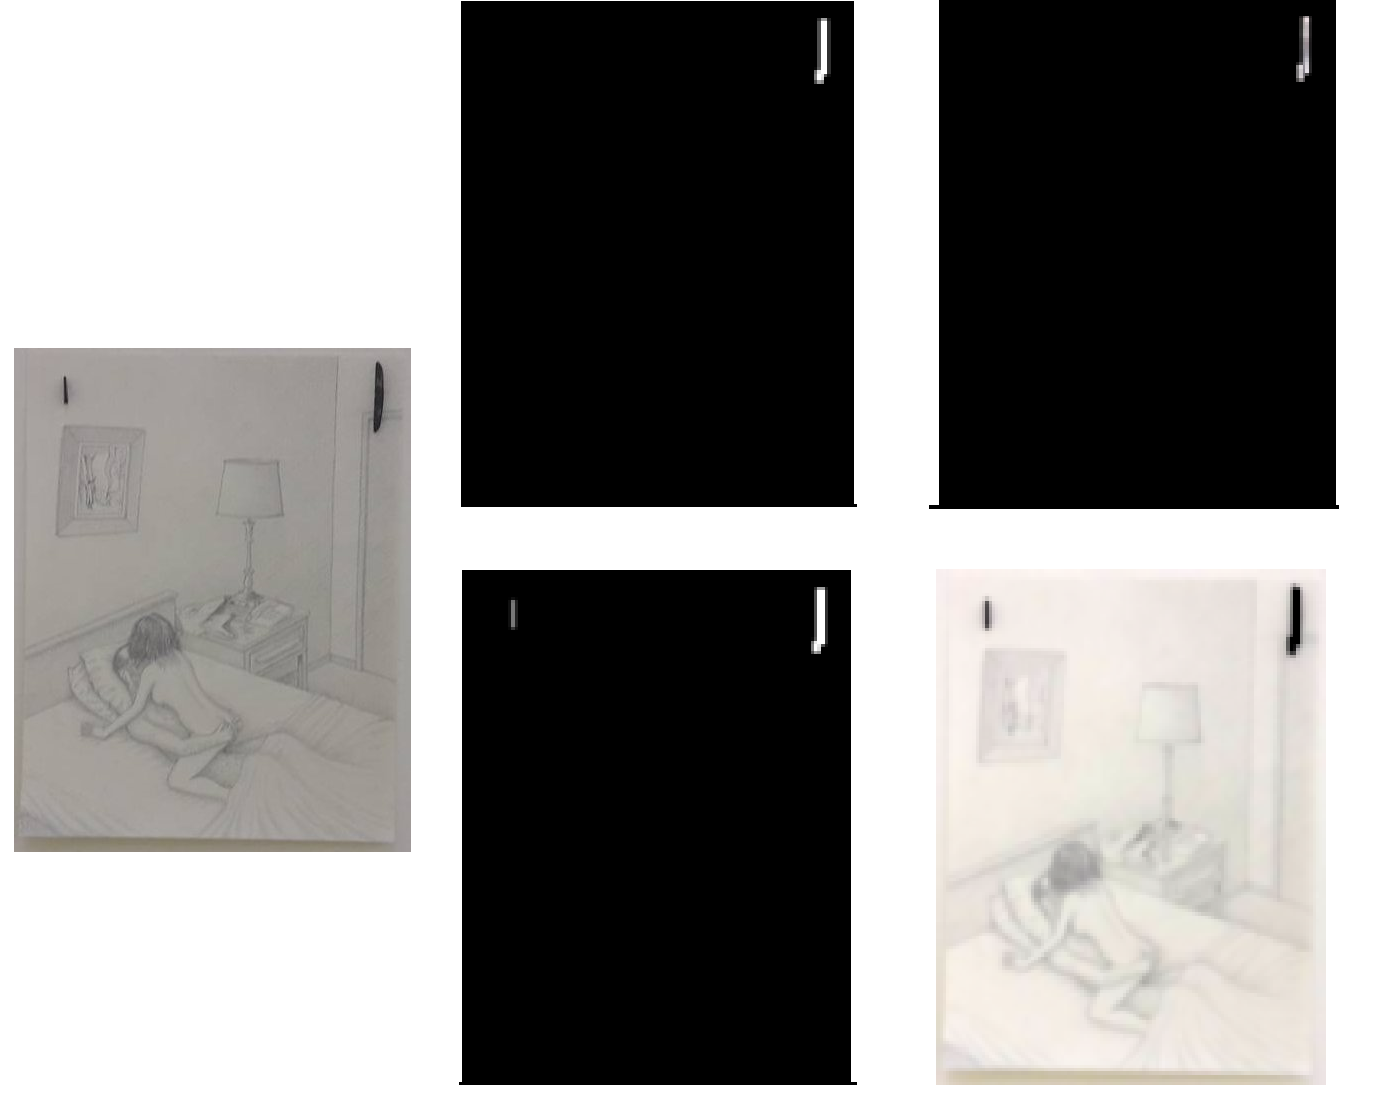
\includegraphics[width=5.5cm]{res_los_amantes.png}}
\center{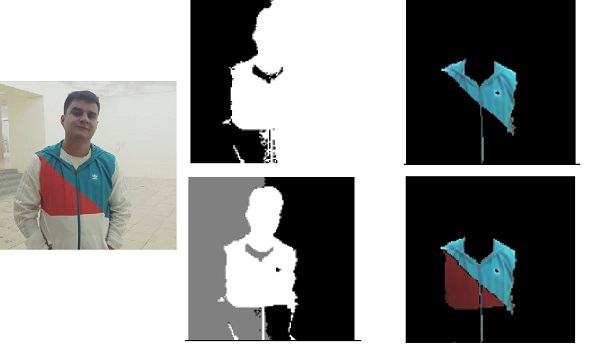
\includegraphics[width=5.0cm]{res_foo.jpg}}
\center{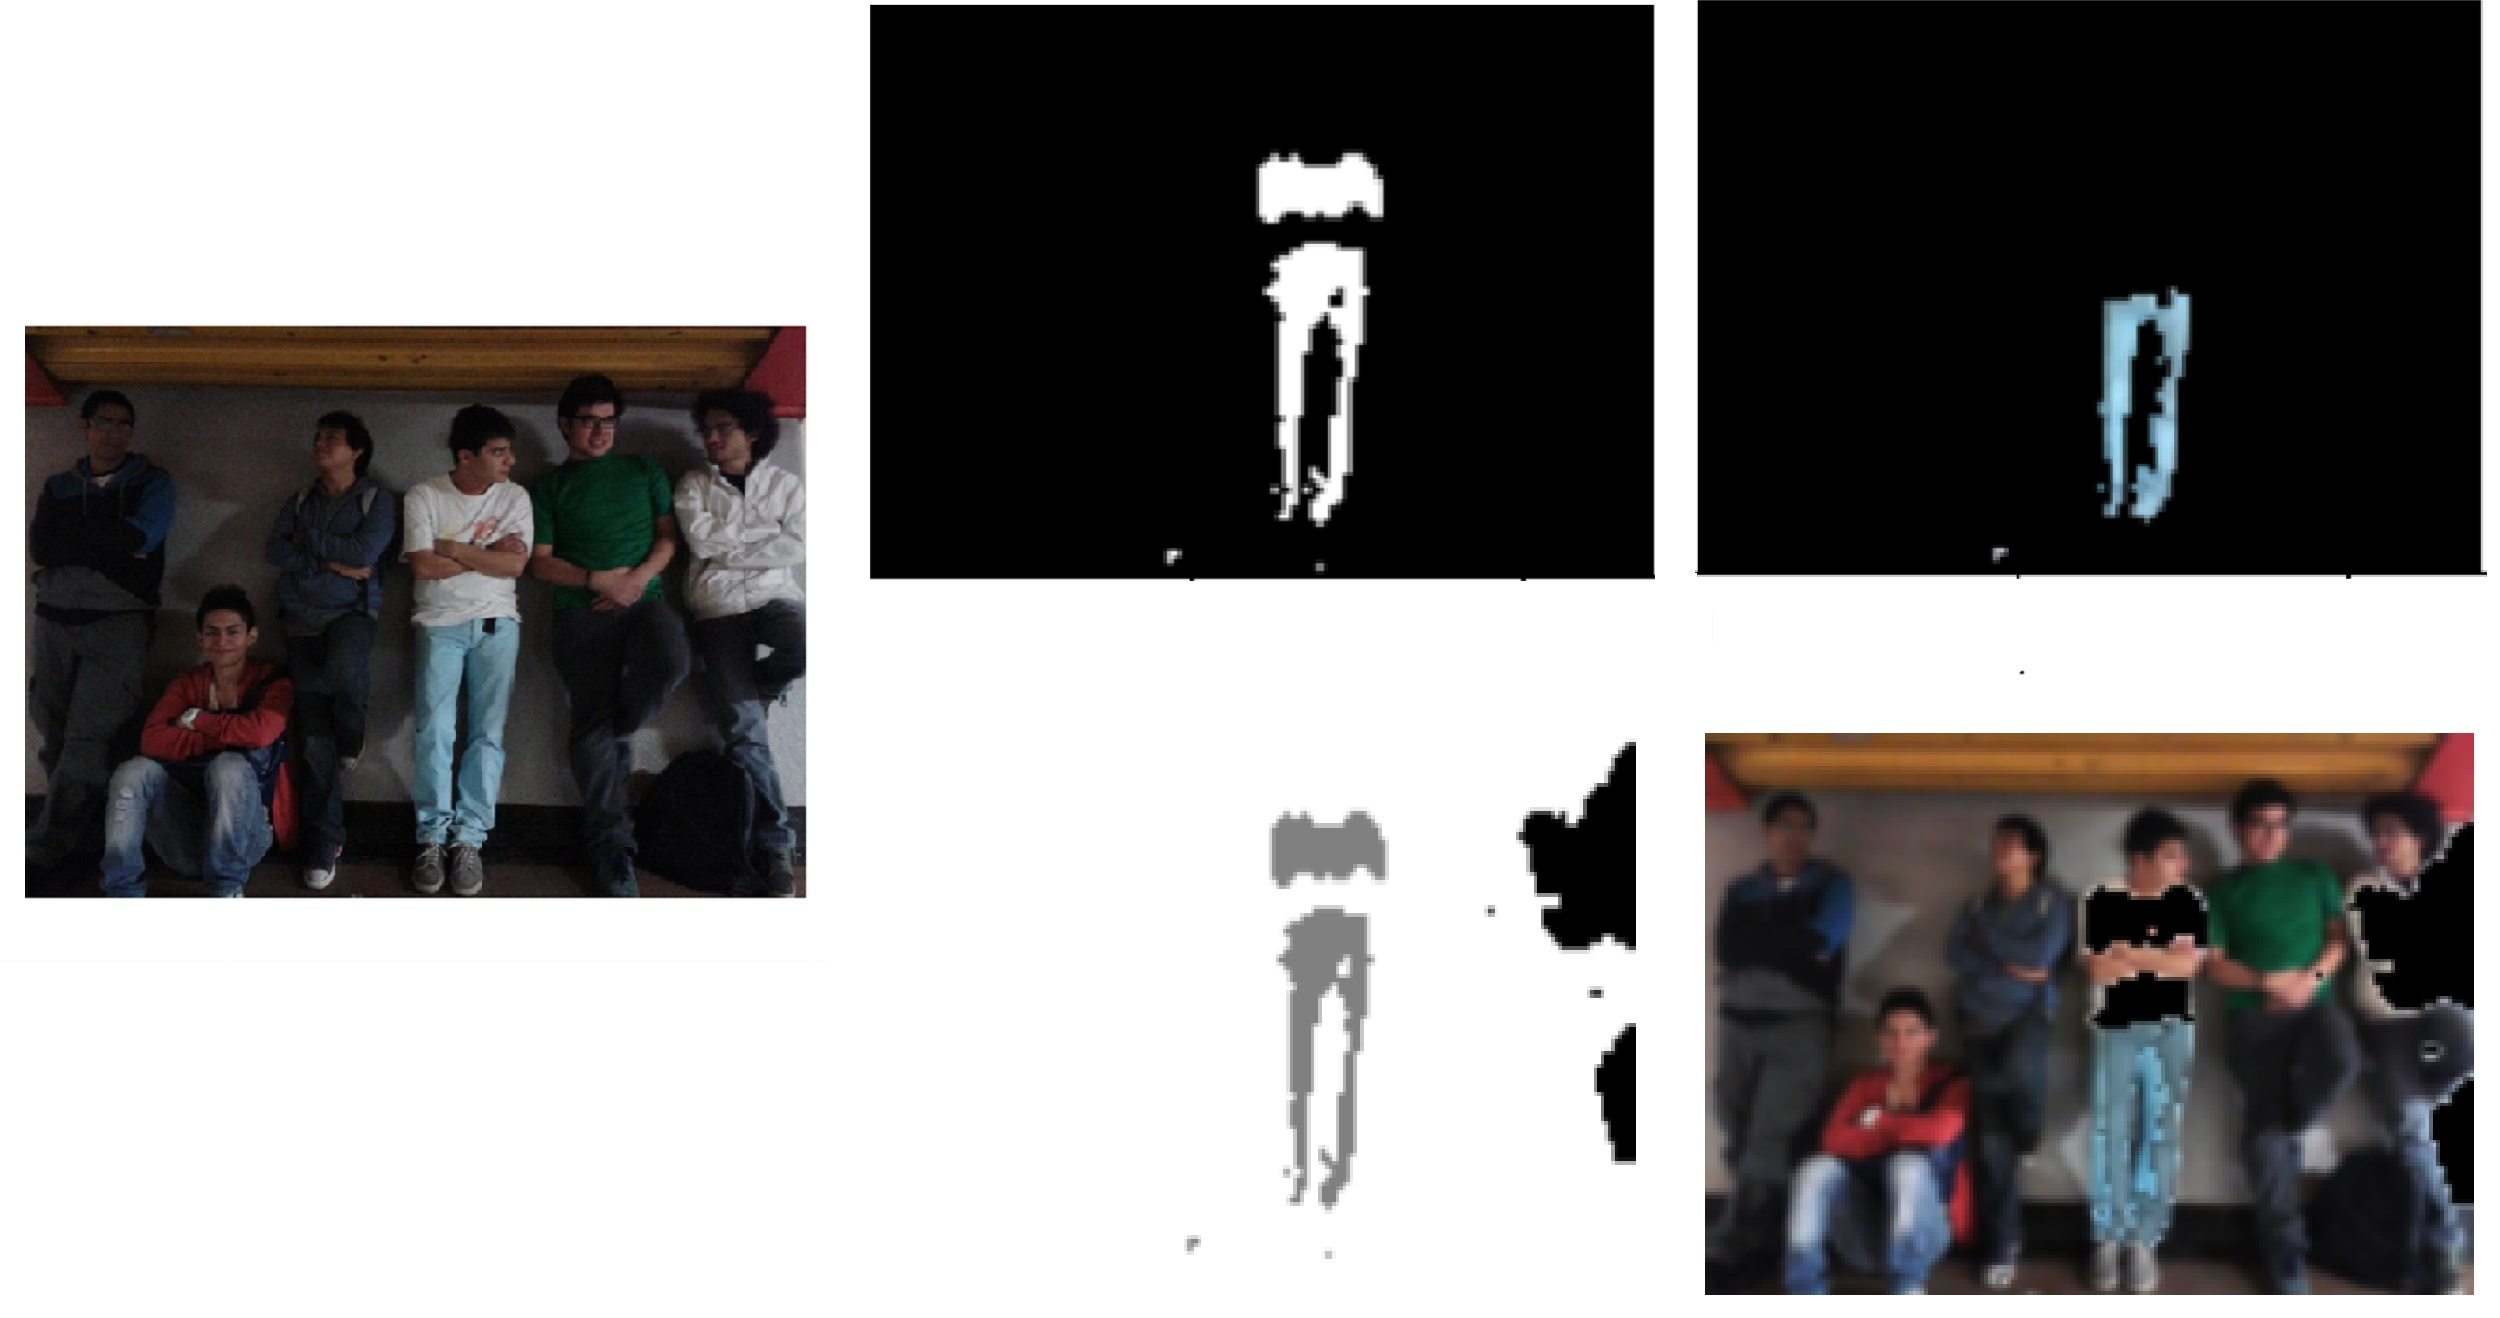
\includegraphics[width=5.0cm]{res_guapa.jpg}}
\center{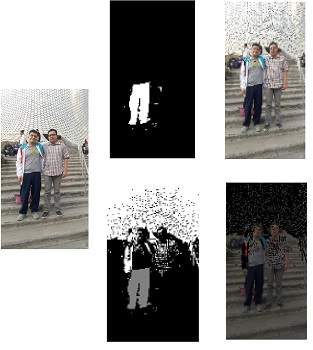
\includegraphics[width=5.0cm]{res_fer.jpg}}
\caption{Results of the segmentation of images 1 to 5, original image (left), segmentation obtained using the eigenvector associated with the second smallest eigenvalue in grayscale and RGB (center and right above) and segmentation obtained using the associated eigenvectors to the second and third smallest eigenvalue in grayscale and RGB (middle and bottom right).}
\label{res1}
\end{figure}
\begin{figure}[htbp]
\center{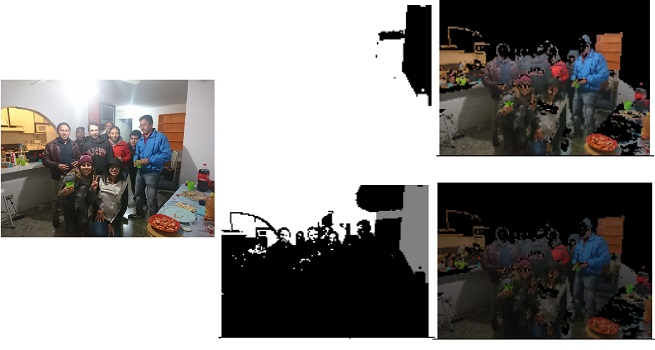
\includegraphics[width=6.3cm]{res_brindis.jpg}}
\center{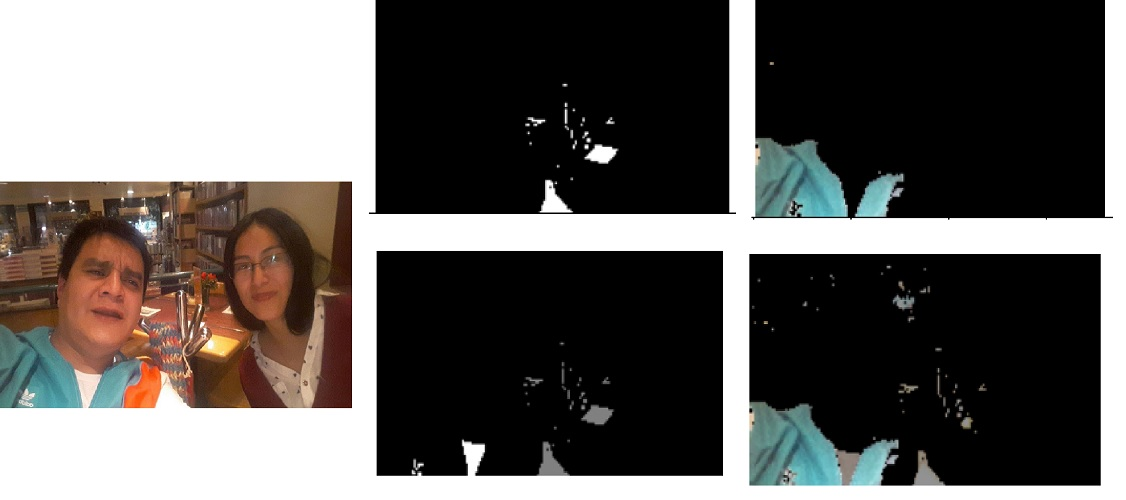
\includegraphics[width=6.3cm]{res_foo_clau.jpg}}
\center{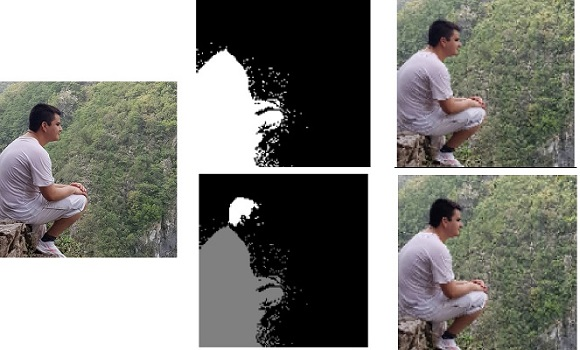
\includegraphics[width=6.3cm]{res_foo2.jpg}}
\center{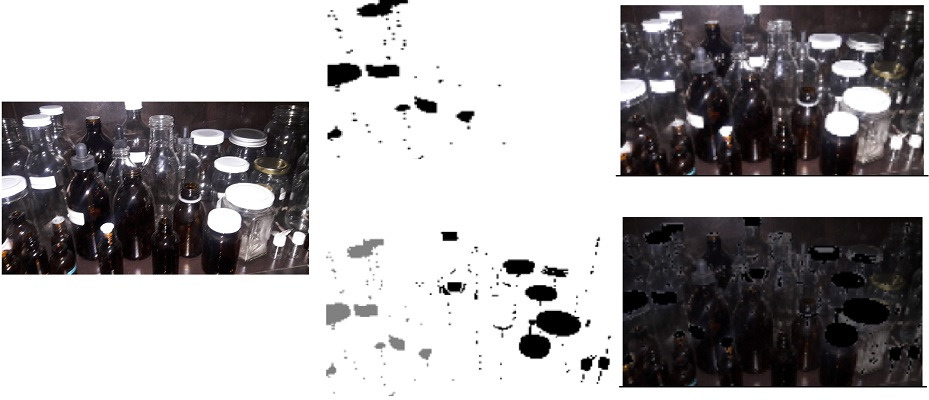
\includegraphics[width=6.3cm]{res_frascos.jpg}}
\center{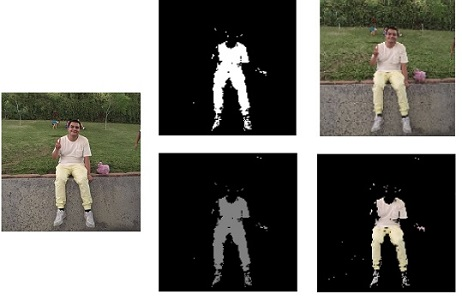
\includegraphics[width=6.3cm]{res_foo3.jpg}}
\caption{Results of the segmentation of images 11 to 14, original image (left), segmentation obtained using the eigenvector associated with the second smallest eigenvalue in grayscale and RGB (center and right above) and segmentation obtained using the associated eigenvectors to the second and third smallest value in grayscale and RGB (middle and bottom right).}
\label{res2}
\end{figure}
\FloatBarrier
\newpage
In figure 4 (from top to bottom) the results obtained through the images 11 to 14 are shown using analogously to figure 2. From the previous set of images we conclude: on the one hand, the image 11 shows that the information provided by the RGB channels is valuable to identify people from the background with a single eigenvector, in counterpoint the images 12 and 13 achieve greater performance in the gray scale (although the image of the butterfly in the RGB channels is easily distinguished). Finally, the image 14 is another sketch, but unlike the image 2, this is a photograph, where we see that the segmentation with the channels in the gray scale achieved a better performance when identifying the body however, this could be due to to causes of lighting at the time of taking the photograph.
\begin{figure}[htbp]
\center{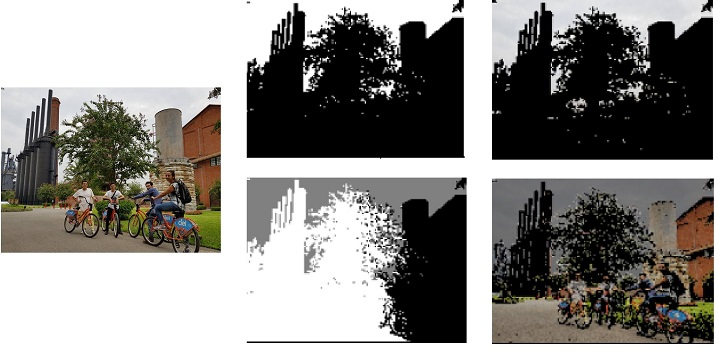
\includegraphics[width=6.65cm]{res_bicis.jpg}}
\center{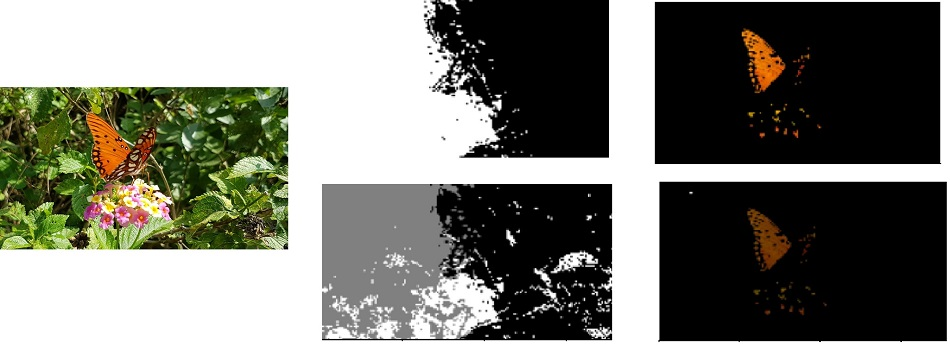
\includegraphics[width=6.6cm]{res_mariposa.jpg}}
\center{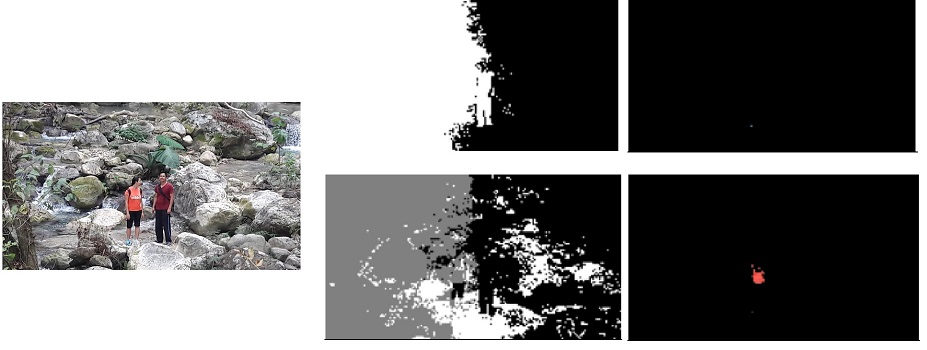
\includegraphics[width=6.6cm]{res_filo_liz.jpg}}
\center{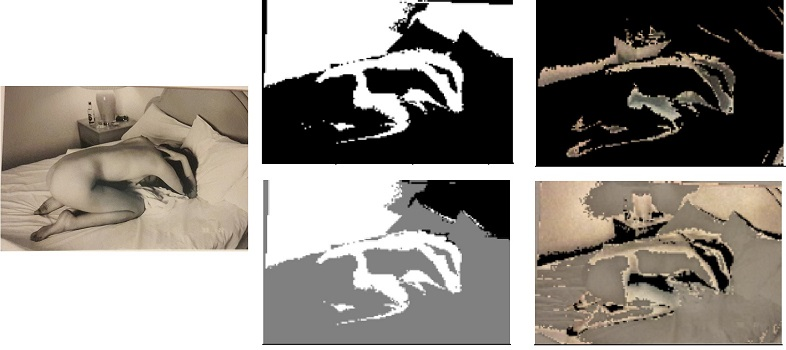
\includegraphics[width=6.65cm]{res_marco.jpg}}
\caption{Results of the segmentation of images 6 to 10, original image (left), segmentation obtained using the eigenvector associated with the second smallest eigenvalue in grayscale and RGB (center and right above) and segmentation obtained using the associated eigenvectors to the second and third eigenvalue smaller in gray scale and RGB (center and right below).}
\label{res2}
\end{figure}
\FloatBarrier
\newpage

\section{Conclusions}
In general terms, what has been learned in the development of this work is: the algorithm \textit {Ncut} presents great potential to segment images (recognize people and variety of materials) as we found in the experiments. In analogy to many other spectral and kernel-based classification methods, such as \textit {string-kernels} or \textit {kernel PCA}, the \textit {Ncut} \textbf {algorithm requires selecting ''appropriately'' a kernel} ( in this case the function we use to construct the \textbf {similarity matrix} $ W $) \textbf {in addition to several parameters} (such as the standard deviations that involve the definition of the kernel used, the way to group pixels from of eigenvectors ...). In counterpoint to the mentioned methods \textit {Ncut} has a \textbf {elegant} formulation that combines basic results of linear algebra and graph theory and their NP property of its exact solution, makes it attractive and \textit {encourages us to subsequent works} to \textbf {evade} the step in the preprocessing that consisted of \ textbf {resize the image}.\\\\\\


\section*{Appendix}

\subsection*{Future works}
As future works, in the first instance we consider avoiding the redimensioning of images and thus experiencing whether considering the image in its entirety provides information that is worth the development and implementation on a large scale (in the short term we consider expanding the implementation to consider inputs from 3000 $ \times $ 3000) even though that means moving the used computing architecture. \\
With the above we will improve the execution times and consider the option to tuning the parameters mentioned in the previous section in order to obtain better results and in the medium plane to make hypotheses about the distribution of such parameters in different domains, or sets of images.
%\begin{displaymath}
%[y]^- = -yI(-y) \textrm{, con } I(-y)=\left\lbrace 
%	\begin{array}{cc}
%	1	&	\textrm{ si } y < 0	\\
%	0	&	\textrm{ otro caso}
%	\end{array} \right.
%\end{displaymath}


%\begin{algorithm}
%{\footnotesize
%\caption{Quadratic Penalty}
%\label{algQuadPen}
%\begin{algorithmic}[1]
%\STATE Given $(\mu_0 > 0$, tolerance $\tau_0$, starting point $x_0^s$
%\FOR{$k=0,1,2\ldots$}
%\STATE Find an approximate minimizer $x_k$ of $Q(\cdot;\mu_k)$, starting at $x_k^s$, and terminating when $||\nabla Q(x;\mu_k)||\leq \tau_k$
%\IF{final convergence test satisfied}
%\STATE \textbf{STOP} with approximate solution $x_k$
%\ENDIF
%\STATE Choose new penalty parameter $\mu_{k+1} \in (0,\mu_k)$
%\STATE Choose new starting point $x_{k+1}^s$
%\ENDFOR
%\end{algorithmic}}
%\end{algorithm}



%{\footnotesize
%\begin{eqnarray}\label{eqgrad}
%\nabla_x \mathcal{L}_A(x_k,\lambda^k;\mu_k) & = & \nabla f(x_k) - \sum_{i\in \mathcal{I}|c_i(x)\leq\mu\lambda_i^k} \left(\lambda_i^k - \frac{c_i(x_k)}{\mu_k} \right) \nabla c_i(x_k)	\nonumber \\
%\end{eqnarray}
%}


%\begin{table}[htbp]
%\begin{center}
%\begin{tabular}{|c|c|c|c|}
%\hline
%			& Penalizaci\'on Cuadr\'atica		&	Barrera Logar\'itmica	&	Lagrangiano Aumentado	\\
%\hline
%$f(x^{*})$	& 0.1643	&	0.1774	&	0.1642	\\
%\hline
%\end{tabular}
%\caption{Resultados para cada m\'etodo en el problema a optimizar.}
%\label{tresults1}
%\end{center}
%\end{table}
\newpage
\begin{thebibliography}{1}
\bibitem{Arpack}
Richard B Lehoucq, Danny C Sorensen, and Chao Yang, \textit{ARPACK users' guide: solution of large-scale eigenvalue problems with implicitly restarted Arnoldi methods}, volume 6. Siam, 1998.

\bibitem{Elixir}
Developmented by José Valim for Plataformatec, \emph{Elixir} , \url{https://elixir-lang.org/}
\bibitem{Facebook}
Facebook Inc, \emph{Facebook}, 2018 and \url{https://www.facebook.com/}

\bibitem{github}
GitHub ,Inc., \emph{GitHub}, 2018 and \url{https://github.com/}

\bibitem{MatrixC}
G.H. Golub and C.F. Van Loan, \emph{Matrix Computations}, John
Hopkins Press, 1989.

\bibitem{MatrixSpark}
Bosagh Zadeh, Reza and Meng, Xiangrui and Ulanov, Alexander and Yavuz, Burak and Pu, Li and Venkataraman, Shivaram and Sparks, Evan and Staple, Aaron and Zaharia, Matei; \textit{Matrix Computations and Optimization in Apache Spark}, Proceedings of the 22Nd ACM SIGKDD International Conference on Knowledge Discovery and Data Mining, KDD '16 2016, ISBN:978-1-4503-4232-2; San Francisco, California, USA; pags 31--38,
\url{http://doi.acm.org/10.1145/2939672.2939675}


\bibitem{Hadoop}
'Welcome to Apache Hadoop!',  \emph{Welcome to Apache Hadoop!}, \url{http://hadoop.apache.org/}. Consulted: 31-Mar-
2018.

\bibitem{imager}
Simon Barthelme (2017). \emph{imager: Image Processing
  Library Based on 'CImg'}, R package version  0.40.2., \url{  https://CRAN.R-project.org/package=imager}

\bibitem{MatLab} 
The MathWorks Inc., \emph{MATLAB}; Natick, Massachusetts, year 2000

\bibitem{ElixirLib}
 Friedel Ziegelmayer, \emph{Matrix}; \url{https://hexdocs.pm/matrix/Matrix.html#summary}, Consulted el 15-Apr-2018


\bibitem{OpenCV}
Bradski, G., \emph{The OpenCV Library}, journal Dr. Dobb's Journal of Software Tools id:2236121, 2008-01-15, year 2000

\bibitem{R}
R Core Team, \emph{R: A Language and Environment for Statistical Computing}, R Foundation for Statistical Computing; Vienna, Austria, 2014 y  \url {http://www.R-project.org/}

\bibitem{Rcpp}
Dirk Eddelbuettel and James Joseph Balamuta (2017). \emph{Extending R with C++: A Brief Introduction to Rcpp}. PeerJ Preprints 5:e3188v1, \url{https://doi.org/10.7287/peerj.preprints.3188v1.}

\bibitem{RcppArmadillo}
Dirk Eddelbuettel, Conrad Sanderson (2014), \emph{RcppArmadillo: Accelerating R with igh-performance C++ linear algebra}, Computational Statistics and Data Analysis, Volume 71, March 2014, pages 1054-1063. \url{
  http://dx.doi.org/10.1016/j.csda.2013.02.005}

\bibitem{RcppEigen}
Douglas Bates, Dirk Eddelbuettel (2013), \emph{Fast and Elegant Numerical Linear Algebra Using the RcppEigen Package}, Journal of Statistical Software, 52(5), 1-24. \url{http://www.jstatsoft.org/v52/i05/}

\bibitem{RSpectra}
Yixuan Qiu and Jiali Mei (2016), \emph{RSpectra: Solvers for Large Scale Eigenvalue and SVD Problems}, R package version 0.12-0, \url{https://CRAN.R-project.org/package=RSpectra}

\bibitem{ScaLAPACK}
Blackford, L. S. and Choi, J. and Cleary, A., D'Azevedo, E. and Demmel, J. and Dhillon, I. and Dongarra, J. and Hammarling, S. and Henry, G. and Petitet, A. and Stanley, K. and Walker, D. and Whaley, R. C.;\emph{ScaLAPACK Users' Guide}, Society for Industrial and Applied Mathematics 1997,
Philadelphia, PA. ISBN :0-89871-397-8  

\bibitem{Ncut}
Shi J. and Malik J., \emph{Normalized Cuts and Image Segmentation}, IEEE Transactions on pattern analysis and machine learning, VOL. 22, No. 8, Ags 2000

\bibitem{Spark}
Spark Community. \emph{Apache Spark},  \url{https://spark.apache.org/}. Consulted: 31-Mar-2018

\bibitem{Sparkbased}
J. Liu, Y. Liang and N. Ansari; \emph{Spark-Based Large-Scale Matrix Inversion for Big Data Processing}; IEEE Access, vol. 4, pp. 2166-2176, 2016, \url{http://ieeexplore.ieee.org/stamp/stamp.jsp?tp=&arnumber=7440788&isnumber=7419931}

\end{thebibliography}


\end{document}

